\chapter{Generacion Exhaustiva acotada desde API de los programas}


\label{cap:beapi}

En adelante, se presenta la técnica desarrollada llamada BEAPI, que tiene como objetivo mejorar la generación exhaustiva acotada (BEG, por sus siglas en inglés, \emph{Bounded Exhaustive Generation}).  Discutiremos las principales ideas de nuestros enfoques para generar de manera eficiente un conjunto exhaustivo acotado de objetos realizando únicamente llamadas a la API de un módulo. Este capítulo está organizado de la siguiente manera: en la Sección \ref{sec:motivating-example}, se presenta un ejemplo que ilustra el problema que se aborda con la técnica propuesta, la cual se explica en la Sección \ref{sec:beapiIntro}. Luego, en las Secciones \ref{sec:scope}, \ref{sec:stateMatching} y \ref{sec:builders}, se describen las optimizaciones implementadas en BEAPI.


\section[Motivación]{Motivación}
\label{sec:motivating-example}

Para motivar las dificultades de escribir especificaciones formales para la generación de estructuras exhaustiva acotadas,  considere el invariante de representación (comúnmente llamados \emph{repOK}) de la clase \emph{NodeCachingLinkedList} (NCL) de Apache, que se muestra en la Figura \ref{fig:NCL-repOK}. Este es un repOK del benchmarks \emph{ROOPS}. Los NCL se componen de una lista principal circular doblemente enlazada, utilizada para el almacenamiento de datos, y una caché de nodos previamente utilizados implementada como una lista enlazada simple. Los nodos eliminados de la lista principal se mueven a la caché, donde se guardan para su uso en el futuro. De esta manera, cuando se requiere un nodo para una operación de inserción, se reutiliza un nodo de la caché (si existe) en lugar de asignar un nuevo nodo. El objetivo es evitar la sobrecarga de recolección de basura para las aplicaciones que realizan una gran cantidad de inserciones y eliminaciones en la lista. El \emph{repOK} devuelve true si y solo si la estructura de entrada satisface las propiedades estructurales de NCL \cite{Liskov00}. Las líneas 1 a 20 verifican que la lista principal sea una lista circular doblemente enlazada con una cabeza ficticia; las líneas 21 a 33 verifican que la caché sea una lista enlazada simple terminada en nulo (y se verifica la consistencia de los campos de tamaño en el proceso). Se observa que repOK está escrito de la manera recomendada por los autores del enfoque de generación exhaustiva de BE, \textsf{Korat} \cite{Boyapati02}. Este devuelve False tan pronto como encuentra una violación de una propiedad prevista en la entrada actual. De lo contrario, devuelve Verdadero al final. Estos repOK permiten a \textsf{Korat} podar grandes porciones del espacio de búsqueda, lo que mejora en gran medida su eficiencia.


\begin{figure}[!thb]
\begin{lstlisting}
public boolean repOK() {
  if (this.header == null) return false;
  //  Missing constraint: the value of the sentinel node
  // must be null  
  // if (this.header.value != null) return false;
  if (this.header.next == null) return false;
  if (this.header.previous == null) return false;
  if (this.cacheSize > this.maximumCacheSize) return false;
  if (this.size < 0) return false;
  int cyclicSize = 0;
  LinkedListNode n = this.header;
  do {
      cyclicSize++;
      if (n.previous == null) return false;
      if (n.previous.next != n) return false;
      if (n.next == null) return false;
      if (n.next.previous != n) return false;
      if (n != null) n = n.next;
  } while (n != this.header && n != null);
  if (n == null) return false;
  if (this.size != cyclicSize - 1) return false;
  int acyclicSize = 0;
  LinkedListNode m = this.firstCachedNode;
  Set visited = new HashSet();
  visited.add(this.firstCachedNode);
  while (m != null) {
      acyclicSize++;
      if (m.previous != null) return false;
      // Missing constraint: the value of cache nodes
      // must be null
      // if (m.value != null) return false;
      m = m.next;
      if (!visited.add(m)) return false;
  }
  if (this.cacheSize != acyclicSize) return false;
  return true;
}
\end{lstlisting}
\caption{\texttt{NodeCachingLinkedList}'s \texttt{repOK} from \textsf{ROOPS}}
\label{fig:NCL-repOK}
\end{figure}

Este ejemplo muestra que escribir \texttt{repOK}s sólidos y precisos para BEG es difícil y consume tiempo. Afinar los \texttt{repOK}s para mejorar el rendimiento de BEG (por ejemplo, para \textsf{Korat}) es aún más difícil. 


\section[BEAPI]{BEAPI}
\label{sec:beapiIntro}

En esta sección discutimos las ideas principales de nuestros enfoques para generar de manera eficiente un conjunto exhaustivo acotado de objetos haciendo solo llamadas a la API de un módulo. Nuestro enfoque se basan en la generación de pruebas dirigida por retroalimentación, explicado en la sección \ref{sec:feedback-directed-test-gen}. 
El enfoque propuesto, denominado \textsf{BEAPI} (Bounded Exhaustive from API), introduce una técnica innovadora para la generación exhaustiva acotada. Este enfoque se basa en la realización de llamadas a las rutinas de la API del software bajo prueba (SUT). Al igual que otros enfoques de generación de pruebas basados en API, \textsf{BEAPI} crea secuencias de llamadas a métodos de la API, conocidas como secuencias de prueba, y las ejecuta para generar estructuras. 

A diferencia de los enfoques de generación basados en caja negra, \textsf{BEAPI} no requiere una especificación formal de las propiedades de las estructuras. En su lugar, el usuario solo debe proporcionar los alcances para la generación, que se abordan en detalle en la sección correspondiente.

La principal ventaja de \textsf{BEAPI} es que requiere un esfuerzo mínimo de especificación para realizar la generación exhaustiva acotada (BEG). Si los métodos de la API utilizados en la generación son correctos, todas las estructuras generadas serán válidas para su construcción. El programador solo necesita asegurarse de que los métodos de la API lancen excepciones cuando se violen las reglas de uso, siguiendo un estilo de programación defensivo \cite{Liskov00}. En la mayoría de los casos, esto implica verificar condiciones muy simples en las entradas. Por ejemplo, el método para agregar (\emph{add(Object)}) un elemento a una \texttt{NCL} lanza una \texttt{IllegalArgumentException} cuando se llama con un elemento \texttt{null}, donde se puede observar que la implementación del método se encarga de cumplir con las demás propiedades del \texttt{NCL}.

Es importante destacar que el enfoque \textsf{BEAPI} aborda las dificultades de escribir especificaciones formales para la generación de estructuras exhaustiva acotadas al aprovechar la ejecución de las rutinas de la API y aplicar técnicas de poda para mejorar la eficiencia de la generación. Esto permite generar estructuras válidas sin requerir una especificación detallada de las propiedades de las estructuras, reduciendo así la carga de trabajo para el programador.

La generación exhaustiva de todas las secuencias de tests factibles a partir de rutinas hasta una longitud máxima, también conocida como generación por fuerza bruta, es un enfoque intrínsecamente combinatorio que consume una gran cantidad de recursos computacionales, incluso para alcances pequeños. Por lo tanto, \textsf{BEAPI} utiliza varias técnicas de poda que son fundamentales para mejorar su eficiencia y permitir la escalabilidad a alcances más grandes.

En primer lugar, \textsf{BEAPI} ejecuta secuencias de prueba y descarta aquellas que producen excepciones que violan las reglas de uso de la API, como \emph{IllegalArgumentException} e \emph{IllegalStateException} en Java.

En segundo lugar, \textsf{BEAPI} implementa la técnica de coincidencia de estado, la cual descarta secuencias de métodos que generan estructuras que ya han sido creadas por secuencias de métodos exploradas previamente. Esta técnica se describe en detalle en la sección correspondiente.

En tercer lugar, \textsf{BEAPI} utiliza un subconjunto de las rutinas de la API para crear las secuencias de prueba. Este subconjunto se identifica mediante un algoritmo de búsqueda greedy y una función de valoración que tiene en cuenta qué subconjunto permite crear la mayor cantidad de objetos utilizando \textsf{BEAPI} en el menor tiempo posible. Este proceso se detalla en el capítulo correspondiente.

A continuación, explicaremos en detalle cada una de estas optimizaciones..

% \cacho{TODO: no se si agregar arbolitos de exploracion para explicarlos}
% \begin{tikzpicture}
%     [level 1/.style={sibling distance=27mm},
%    level 2/.style={sibling distance=25mm},
%    every node/.style={rectangle,draw,fill=white,minimum size=10mm,align=center,font=\tiny},
%    edge from parent/.style={draw}]
   
%   % Raíz
%   \node {n = new NCL()}
%     % Hijos
%     child {node {n = new NCL() \\
%                 n.add(int)}
%       child {node {n = new NCL() \\
%                     n.method()}}
%       child {node {n = new NCL() \\
%                     n.anotherMethod()}}
%     }
%    child {node {n = new NCL() \\
%                 n.addFirst()}}
%    child {node {n = new NCL() \\
%                 n.remove()}}
%     child {node {...}}
%     % child {node {Método N}};
% \end{tikzpicture}



\section{Scope}
\label{sec:scope}

\begin{figure}[H]
    \centering
    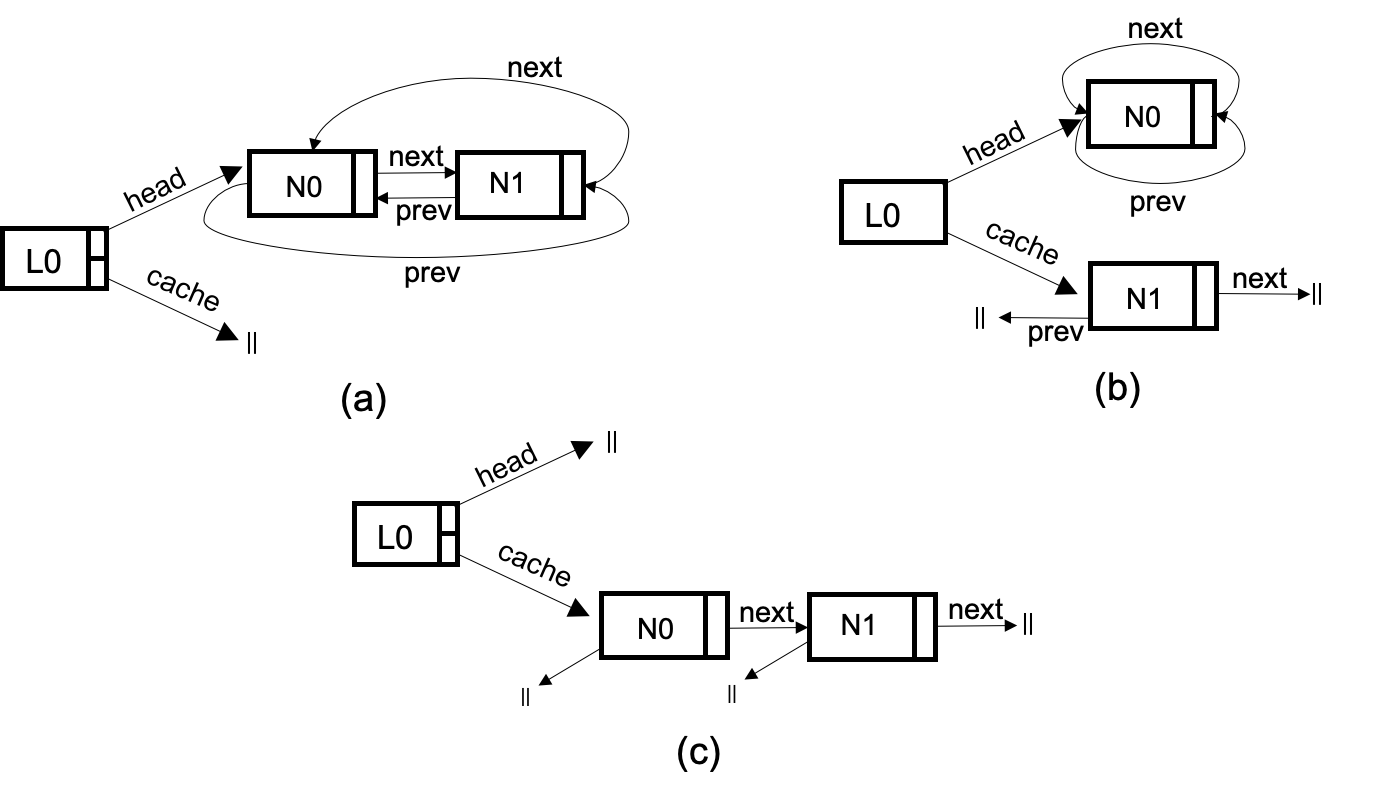
\includegraphics[width=0.85\textwidth]{NCL-instances.png}
    \caption{Tres instancias de NodeCachingLinkedList con exactamente dos nodos}
    \label{fig:ncl-instances}
\end{figure}


Lo primero que realizamos fue adaptar nuestra técnica basada en generación de test basada por feedback para que funcione con un conjunto fijo de valores primitivos (enteros del 0 al $k-1$). (Normalmente, las técnicas basada en generación por retroalimentación guardaría los valores primitivos que son devueltos por la ejecución de las pruebas y reutilizaría estos valores en pruebas futuras). También logramos descartar secuencias de métodos que crean objetos con más de $k$ objetos (de cualquier tipo), para evitar que se construyan objetos más grandes de lo necesario. Para lograr esto, canonizamos los objetos generados por la ejecución de cada secuencia y descartamos la secuencia si algún objeto tiene un índice igual o mayor que $k$.

\begin{figure}[H]
\begin{lstlisting}[keywordstyle=\scriptsize\ttfamily]
max.objects=3
int.range=0:2
strings=str1,str2,str3
omit.fields=NCL.DEFAULT_MAXIMUM_CACHE_SIZE
\end{lstlisting}
\caption{\textsf{BEAPI}'s scope definition for \texttt{NCL} (max. nodes 3)}
\label{fig:NCL-fin-BEAPI}
\end{figure}

\emph{BEAPI} explora el espacio de búsqueda de secuencias de prueba (acotadas) que se pueden formar mediante llamadas a la API. Supongamos el caso de la figura \ref{fig:ncl-instances} de instancias de \texttt{NCL}.  El límite $k$ representa el número máximo de objetos que se pueden crear para cada clase (en la Figura \ref{fig:ncl-instances}, el número de nodos en los objetos NCL está acotado por $k=2$) y el número máximo de valores primitivos disponibles (por ejemplo, enteros del 0 a $k-1$). Esto asegura que se generen NCL con no más de 2 nodos. 
Por lo tanto, debemos proporcionar dominios de datos para los tipos primitivos utilizados en esas llamadas y establecer un límite en el tamaño máximo de las estructuras que deseamos generar a partir de esas llamadas de API. Para limitar el número de estructuras generadas y establecer los valores primitivos, BE necesita un archivo de descripción simple en formato \texttt{java.properties}, en el que se establecen algunos parámetros. (Figura \ref{fig:NCL-fin-BEAPI}).  La línea 1 del archivo de configuracion de \emph{BEAPI} establece el número máximo de objetos que se asignarán para cada clase, en este caso es 2. Esto especifica el número máximo de objetos diferentes (alcanzables desde la raíz) permitidos en una estructura. Las secuencias de prueba generadas por \emph{BEAPI} que crean estructuras que exceden este número (para cualquier clase) se descartan y no se extienden aún más. Esto asegura que se generen solo \texttt{NCL} con no más de 2 nodos. La línea 2 especifica que solo se emplearán enteros del 0 al 2 para invocar rutinas de la API que tomen valores enteros como parámetros (es decir, para insertar un entero en la lista, eliminar un entero, insertar en una posición entera dada, etc.). También se puede especificar dominios para otros tipos primitivos como floats, doubles y strings (linea 3) describiendo sus valores por extensión. Podemos indicarle a \emph{BEAPI} que ignore algunos campos en el proceso de canonización de objetos, que se lleva a cabo en la ejecución de las secuencias de métodos de la API. Esto permite al usuario controlar qué partes de la estructura del objeto son relevantes para la coincidencia de estados (ver más adelante en la sección \ref{sec:stateMatching}). Por ejemplo,  la línea 4 haría que \emph{BEAPI} omita el tamaño máximo predeterminado de la caché en la coincidencia de estados, que en la API de \emph{NCL} es una constante inicializada en 20 en el constructor de la clase. Es importante que aqui se omitan campos que puede afectar la coincidencia de estados, como el caso del campo \emph{modCount}. Esta variable se utiliza a menudo en estructuras de datos para realizar un seguimiento de las modificaciones o cambios realizados en los datos almacenados, pero claramente no afecta la estructura generada. 
La configuración mostrada en la Figura~\ref{fig:NCL-fin-BEAPI} es suficiente para que \emph{BEAPI} genere NCL con un máximo de 3 nodos, que contienen enteros del 0 al 2 como valores. 
\\
% \begin{figure}[h!]
%     \centering
%     \begin{verbatim}
% max.objects = 3
% int.range = 0, 2
% str1 = "value1"
% str2 = "value2"
% str3 = "value3"
% omit.fields = maxCacheSize, modCounts
%     \end{verbatim}
%     \caption{Archivo de configuración de \textsf{BEAPI} para el estudio de caso de \texttt{NCL}}
%     \label{fig:NCL-fin-BEAPI}
% \end{figure}

\section{State Matching}
\label{sec:stateMatching}

En la generación de pruebas con \textsf{BEAPI}, a menudo muchas secuencias de prueba producen la misma estructura. Por ejemplo, insertar un elemento en una lista y luego eliminarlo. \textsf{BEAPI} asume que las ejecuciones de métodos son deterministas, es decir, cualquier ejecución de una rutina con las mismas entradas produce los mismos resultados. Observamos que para cada estructura distinta $s$, solo necesitamos guardar la primera secuencia de prueba que genera $s$ (y la estructura en sí). Todas las secuencias de prueba generadas posteriormente que también crean $s$ pueden ser descartadas. Si almacenamos muchas secuencias de prueba para la misma estructura, todas estas secuencias tendrían que ser extendidas con nuevas rutinas en iteraciones posteriores de \textsf{BEAPI}, lo que resultaría en extensiones innecesarias. Por lo tanto, implementamos la coincidencia de estados en \textsf{BEAPI} de la siguiente manera.

Almacenamos todas las estructuras producidas hasta ahora por \textsf{BEAPI} en una forma canónica (ver más abajo). Después de ejecutar la última rutina \texttt{r(p$_1$, ..., p$_k$)} de una nueva secuencia de prueba generada \texttt{T}, comprobamos si alguno de los parámetros de \texttt{r} tiene una estructura no vista antes (no almacenada). Si \texttt{T} no crea ninguna estructura nueva, se descarta. De lo contrario, \texttt{T} y las nuevas estructuras que genera son almacenadas por \textsf{BEAPI}.

Representamos las estructuras asignadas en el heap como grafos etiquetados. Después de la ejecución de un método, un parámetro $p$ (de tipo no primitivo) contiene una referencia al objeto raíz $r$ de un montículo con raíz (es decir, $p=r$), definido a continuación.

\begin{definition}
Sea $O$ un conjunto de objetos y $P$ un conjunto de valores primitivos (incluido $null$). Sea $F$ el conjunto de campos de todos los objetos en $O$.
\begin{itemize}
\item Un \emph{heap} es un grafo etiquetado $H = \langle O, E\rangle$ con $E = {(o, f, v) | o \in O, f \in F, v \in O \cup P}$.
\item Un \emph{heap con raíz} es un par $RH = \langle r, H \rangle$ donde $r \in O$, $H = \langle O, E\rangle$ es un heap, y para cada $v' \in O \cup P$, $v'$ es alcanzable desde $r$ a través de campos en $F$.
\end{itemize}
\end{definition}

El caso especial $p = null$ se puede representar con un montículo con raíz que tiene un nodo ficticio y un campo ficticio que apunta a null. En lenguajes como Java, cada objeto se identifica por la dirección de memoria donde se encuentra. Cambiar las direcciones de memoria donde se asignan los objetos no tiene efecto desde el punto de vista del programa, ya que el programador no tiene control sobre la representación de bajo nivel de la memoria (a diferencia de otros lenguajes como C). Los montículos obtenidos mediante permutaciones de las direcciones de memoria de sus objetos componentes se llaman \emph{heaps isomorfos}. Evitamos la generación de \emph{heaps isomorfos} empleando una representación canónica para los heaps \cite{Iosif02,Boyapati02}. Los heaps con raíz se pueden canonizar eficientemente mediante un enfoque llamado \emph{linearización} \cite{Iosif02,Xie04}, que transforma un heap con raíz en una secuencia única de valores.

\bigbreak

\begin{figure}[!th]
\begin{lstlisting}
int[] linearizar(O raiz, Heap<O, E> heap, int alcance, Regex omitirCampos) {
    Map ids = new Map(); // mapea nodos a sus identificadores unicos
    return lin(raiz, heap, alcance, ids, omitirCampos);
}
int[] lin(O raiz, Heap<O, E> heap, int alcance, Map ids, Regex omitirCampos) {
    if (ids.containsKey(raiz))
        return secuenciaUnica(ids.get(raiz));
    if (ids.size() == alcance)
        throw new ExcepcionAlcanceSuperado();
    int id = ids.size() + 1;
    ids.put(raiz, id);
    int[] seq = secuenciaUnica(id);
    Edge[] campos =
    ordenarPorCampo({ <raiz, f, o> en E }, omitirCampos);
    foreach (<raiz, f, o> en campos) {
        if (esPrimitivo(o))
            seq.add(representacionUnica(o));
        else
            seq.append(lin(o, heap, alcance, ids, omitirCampos));
    }
    return seq;
}
\end{lstlisting}
\caption{Algoritmo de linearización}
\label{alg:linearization}
\end{figure}


El algoritmo mostrado en la Figura~\ref{alg:linearization} es una versión personalizada para \textsf{BEAPI} del algoritmo de linearización presentado en \cite{Xie04}. Esta versión ha sido modificada para informar cuando los objetos exceden los alcances y para admitir la omisión de campos de objeto.

El algoritmo \texttt{linearize} invoca a la función \texttt{lin} y realiza un recorrido en profundidad del heap comenzando desde la raíz (línea 3). Durante este recorrido, se asignan identificadores de objeto diferentes a cada objeto visitado. Cuando se visita un objeto por primera vez, se le asigna un nuevo identificador único (líneas 10-11) y se crea una secuencia de un solo elemento llamada \texttt{seq}, que contiene el identificador de objeto y representa el objeto (línea 12). El mapa \texttt{ids} se utiliza para almacenar el mapeo entre los objetos y los identificadores de objeto únicos.

A continuación, se recorren los campos del objeto en un orden predefinido (por ejemplo, por nombre) y se construye la linearización de cada valor de campo, que se agrega a la secuencia \texttt{seq} (líneas 13-19). Si un campo almacena un valor primitivo (línea 15), se agrega una secuencia de un solo elemento que representa ese valor a \texttt{seq} (línea 16). Si el campo hace referencia a otro objeto, se realiza una llamada recursiva a la función \texttt{lin} para transformarlo en una secuencia, que luego se agrega a \texttt{seq} (línea 18).

Al final del bucle, la secuencia \texttt{seq} contiene la representación canónica de todo el heap que comienza en la raíz, y se devuelve por la función \texttt{lin} (línea 20). Sin embargo, si se encuentra un objeto que ya ha sido visitado en llamadas recursivas anteriores, es decir, que ya tiene un identificador asignado en \texttt{ids}, el algoritmo devuelve una secuencia de un solo elemento que contiene el identificador único del objeto (líneas 6-7).

Si hay más de \texttt{scope} objetos alcanzables desde el heap enraizado, lo cual significa que se ha superado el límite de alcances establecido, el algoritmo \texttt{linearize} devuelve una excepción para informar esta situación (líneas 9-10). Además, el parámetro \texttt{linearize} también acepta una expresión regular llamada \texttt{omitFields}, que se utiliza para coincidir con los nombres de los campos que deben ser omitidos durante la canonicación del heap.

Para omitir dichos campos, se implementa la función \texttt{sortByField} (línea 13) de manera que no se devuelven las aristas correspondientes a los campos cuyos nombres coinciden con \texttt{omitFields}. Es importante destacar que este comportamiento es específico de nuestro enfoque, ya que la excepción será utilizada por \textsf{BEAPI} para descartar secuencias de prueba que generen objetos que excedan los alcances permitidos.

Cabe destacar que la linearización proporciona una forma eficiente de comparar objetos: dos objetos se consideran iguales si y solo si las secuencias correspondientes generadas por la función \texttt{linearize} son iguales.


\section{Uso de Builders en BEAPI}
\label{sec:builders}
En esta sección, introducimos una optimización que hemos desarrollado y que es una parte importante de esta tesis. Explicaremos una de las formas en las que utilizamos una técnica llamada \emph{identificación de métodos builders} en una API. Estos métodos builders nos permiten generar una gran diversidad de objetos (pudiendo generar de manera exhaustiva, es decir, generando todos los objetos posibles hasta un alcance dado).

Dado que la cantidad de combinaciones factibles de métodos crece de manera exponencial con el número de métodos, es crucial reducir la cantidad de métodos que \textsf{BEAPI} utiliza para producir secuencias de prueba. Para abordar este problema, utilizamos un enfoque de identificación automática de métodos builders que se describe en el capítulo siguiente (Capítulo \ref{cap:builders}). Este enfoque nos ayuda a encontrar un subconjunto de métodos de la API que son suficientes para generar conjuntos de estructuras acotadas y exhaustivas. En el contexto de \textsf{BEAPI}, utilizamos un algoritmo de búsqueda de tipo Greedy para identificar este subconjunto de builders.

En esta sección, presentamos un enfoque más simple basado en el algoritmo de optimización Hill Climbing (HC) que logra un mejor rendimiento. Aunque HC puede ser menos preciso, ya que puede incluir algunos métodos que no son necesarios para producir un conjunto acotado y exhaustivo de estructuras, en nuestros experimentos, HC funcionó muy bien y calculó consistentemente conjuntos mínimos de builders (verificamos que coincidieran con los builders identificados manualmente en cada estudio de caso). Nuestro objetivo aquí es evaluar el impacto de utilizar builders para la generación exhaustiva acotada (BEG) a partir de una API.

Para la identificación de métodos builders, utilizamos una función de evaluación que emplea un generador exhaustivo para crear objetos de la API (ver sección \ref{sec:fitness}). El algoritmo Hill Climbing realiza múltiples invocaciones a este generador exhaustivo durante la identificación de los builders.

La idea clave que hace posible la identificación de builders es que a menudo los builders identificados para un alcance relativamente pequeño son los mismos que se necesitan para crear estructuras de cualquier tamaño. En otras palabras, una vez que el alcance es lo suficientemente grande para calcular los builders, aumentar aún más el alcance no modificará el conjunto de builders. Este resultado se asemeja a la hipótesis del alcance pequeño para la detección de errores \cite{Andoni02} (y a la técnica de "transcoping" \cite{Rosner13}). En todos nuestros casos de estudio, un alcance de 5 fue suficiente para calcular los builders (verificamos manualmente la corrección de los builders en todos los casos). Después de identificar eficientemente los builders con un alcance pequeño, podemos ejecutar \textsf{BEAPI} utilizando los builders identificados y un alcance mayor. Esto nos permite generar objetos más grandes y utilizarlos para probar el SUT.

En la mayoría de nuestros casos de estudio, los builders consisten en un constructor y un solo método para agregar elementos a la estructura. Sin embargo, nuestro enfoque automatizado de identificación de builders mostró que, en el caso de los árboles Rojo-Negro, también se requería un método de eliminación (para alcances mayores que 3). Esto se debe a que existen árboles con una configuración específica de equilibrio (coloreando los nodos en rojo y negro) que no se pueden construir solo agregando elementos al árbol. En contraste, los árboles AVL, que también son estructuras balanceadas, no requieren el método de eliminación como parte de su builder; solo el constructor de la clase y una rutina de adición son suficientes. Esto demuestra que la identificación de builders no es trivial de realizar manualmente.

Para obtener más información sobre esta sección, invitamos al lector a leer el siguiente capítulo donde se explica en detalle el desarrollo de esta técnica (Capítulo \ref{cap:builders}).

\section{Algoritmo de BEAPI}
\label{sec:beapiTechnique}

A continuación se muestra un pseudocódigo de \emph{BEAPI} en la Figura \ref{alg:beapi}. \emph{BEAPI} toma como entradas una lista de métodos de una API,  \texttt{methods}. Estos metodos pueden ser la API completa o un subconjuntos de metodos de la misma. En nuestro caso, como hemos aplicado anteriormente, vamos a utilizar los métodos \emph{builders} previamente identificados. Ademas, es algoritma toca el alcance (scope) de objetos para la generación, \texttt{scope}; una lista para crear valores de cada tipo primitivo proporcionado en la descripción del alcance, \texttt{primitives} (creados automáticamente a partir de las opciones de configuración como \texttt{int.range}, \texttt{string}, etc., ver Figura~\ref{fig:NCL-fin-BEAPI}); y una expresión regular que coincide con los campos que se deben omitir en la canonicación de las estructuras, \texttt{omitFields}. Observa que se pueden pasar métodos de más de una clase en \texttt{methods} si se desean generar objetos para varias clases en la misma ejecución de \textsf{BEAPI}, por ejemplo, cuando los métodos de una clase toman objetos de otra clase como parámetros. La estructura de datos de tipo Map, \texttt{currSeqs} de \emph{BEAPI}  almacena, para cada tipo, la lista de secuencias de test que se sabe que generan estructuras del tipo correspondiente. El \cacho{check}\texttt{currSeqs} se inicia con todas las secuencias de tipos primitivos en \texttt{primitives} (líneas 3-4). En cada iteración del bucle principal (líneas 6-39), \textsf{BEAPI}  crea nuevas secuencias para cada método disponible \texttt{m} (línea 9), explorando exhaustivamente todas las posibilidades para crear secuencias de prueba utilizando \texttt{m} e inputs generados en iteraciones anteriores y almacenados en \texttt{currSeqs} (líneas 10-35). Las secuencias de prueba recién creadas que generan nuevas estructuras en la iteración actual se guardan en el mapa \texttt{newSeqs} (inicializado vacío en la línea 7). Se puede observar que todas las secuencias generadas se agregan a \texttt{currSeqs} al final de la iteración principal (línea 40). Si no se producen nuevas estructuras en la iteración actual (\texttt{newStrs} es falso en la línea 36), el bucle principal del algoritmo de  \textsf{BEAPI}  termina su ejecución y se devuelve la lista de todas las secuencias en \texttt{currSeqs} (línea 40).


\begin{figure}[t!]

\begin{lstlisting}[language=Java]
public BEAPI(List methods, int scope, Map<Type, List<Seq>> primitives, 
Regex omitFields) {
    Map<Type, List<Seq>> currSeqs = new Map();
    currSeqs.addAll({ T->L | T->L in primitives });
    Set canonicalStrs = new Set();
    for (int it=0; true; it++) {
      Map<Type, List<Seq>> newSeqs = new Map();
      boolean newStrs = false;
      for (m(T1,...,Tn):Tr: methods) {
        Map<Type, List<Seq>> seqsT1 = currSeqs.getSequencesForType(T1);
        ...
        Map<Type, List<Seq>> seqsTn = currSeqs.getSequencesForType(Tn);
        for ((s1,...,sn): seqsT1 x ... x seqsTn) {
          Seq newSeq = createNewSeq(s1,...,sn,m);
          o1,...,on,or,failure,exception = execute(newSeq);
          if (failure) 
            throw new ExecutionFailedException(newSeq);
          if (exception) 
            continue;
          c1,...,cn,cr,outOfScope = makeCanonical(o1,...,on,scope,omitFields);
          if (outOfScope) 
            continue;
          if (isReferenceType(T1) and !canonicalStrs.contains(c1)) {
                canonicalStrs.add(c1);
                newSeqs.addSeqForType(T1, newSeq);
                newStrs = true;
          }
          ...
          if (isReferenceType(Tr) and !canonicalStrs.contains(cr)) {
                canonicalStrs.add(cr);
                newSeqs.addSeqForType(Tr, newSeq);
                newStrs = true;
          }
        }
      }
      if (!newStrs) 
        break;
      currSeqs.addAll(newSeqs);
    }
    return currSeqs.getAllSeqsAsList();
}
\end{lstlisting}
\caption{\textsf{BEAPI} algorithm}
\label{alg:beapi}
\end{figure}

A continuación, comentaré los detalles del bucle for en las líneas 9-35. En primer lugar, se obtienen todas las secuencias que se pueden utilizar para construir entradas para \texttt{m} en \texttt{seqsT$_1$}, ..., \texttt{seqsT$_n$}. \textsf{BEAPI} explora cada tupla \texttt{(s$_1$}, ..., \texttt{s$_n$)} de entradas factibles para \texttt{m}. A continuación, se ejecuta \texttt{createNewSeq} (línea 14), que construye una nueva secuencia de prueba \texttt{newSeq} realizando la composición secuencial de las secuencias de prueba \texttt{s$_1$}, ..., \texttt{s$_n$} y la rutina \texttt{m}, y reemplazando los parámetros formales de \texttt{m} por las variables que crean los objetos requeridos en \texttt{s$_1$}, ..., \texttt{s$_n$}. Luego, se ejecuta \texttt{newSeq} (línea 15) y como resultado podemos tener que, produzca un fallo (\texttt{failure} se establece en verdadero), genera una excepción que representa un uso no válido de la API (\texttt{exception} se establece en verdadero) o su ejecución tiene éxito y crea nuevos objetos \texttt{o$_1$,$\ldots$,o$_n$}. En caso de fallo, se lanza una excepción y \texttt{newSeq} se presenta al usuario como evidencia del fallo (línea 17). Si se lanza un tipo diferente de excepción, \textsf{BEAPI} asume que corresponde a un mal uso de la API (ver más abajo), descarta la secuencia de prueba (línea 19) y continúa con la siguiente secuencia candidata. De lo contrario, la ejecución de \texttt{newSeq} genera nuevos objetos \texttt{o$_1$,$\ldots$,o$_n$} (o valores de tipos primitivos) que se canonizan mediante \texttt{makeCanonical} (línea 20) --ejecutando \texttt{linearize} de la Figura~\ref{alg:linearization} en cada estructura. Si alguna de las estructuras producidas por \texttt{newSeq} excede el scope, \texttt{makeCanonical} establece \texttt{outOfScope} en verdadero, \textsf{BEAPI} descarta \texttt{newSeq} y continúa con la siguiente (línea 22).
Esto garantiza que \textsf{BEAPI} nunca crea objetos más grandes que el scope dado.
Si ninguna de las situaciones anteriores ocurre, quiere decir que ha pasado todos los chequeos la secuencia corriente y, \texttt{makeCanonical} devuelve versiones canónicas de \texttt{o$_1$,$\ldots$,o$_n$} en las variables \texttt{c$_1$,$\ldots$,c$_n$}, respectivamente. A continuación, \textsf{BEAPI} realiza una coincidencia de estado comprobando que la estructura canónica \texttt{c$_1$} sea de tipo de referencia y que no haya sido creada por ninguna secuencia de prueba anterior (línea 23). Observa que \texttt{canonicalStrs} almacena todas las estructuras ya visitadas. Si \texttt{c$_1$} es una nueva estructura, se agrega a \texttt{canonicalStrs} (línea 24) y se agrega la secuencia que crea \texttt{c$_1$}, \texttt{newSeq}, al conjunto de secuencias de prueba que producen estructuras de tipo \texttt{T$_1$} (\texttt{newSeqs} en la línea 27). Además, se establece \texttt{newStrs} en verdadero para indicar que al menos se ha creado un nuevo objeto en la iteración actual (línea 26). Este proceso se repite para los objetos canónicos \texttt{c$_2$,$\ldots$,c$_n$,c$_r$} (líneas 29-32).
\cacho{Un for aqui}

\textsf{BEAPI} distingue los fallos del mal uso de la API en función del tipo de excepción (similarmente a las técnicas anteriores de generación de pruebas basadas en API \cite{Pacheco07}). Por ejemplo,\\
\texttt{IllegalArgumentException} y \texttt{IllegalStateException} corresponden a usos incorrectos de la API, y el resto de las excepciones se consideran fallos de manera predeterminada. La implementación de \textsf{BEAPI} permite al usuario seleccionar las excepciones que corresponden a fallos y aquellas que no, configurando los parámetros correspondientes. Como se mencionó en la Sección~\ref{sec:motivating-example}, \textsf{BEAPI} asume que los métodos de la API lanzan excepciones cuando no se pueden ejecutar con entradas inválidas. Sostenemos que esta es una práctica común, llamada programación defensiva \cite{Liskov00}, que todos los programadores deberían seguir, ya que resulta en un código más robusto y mejora las pruebas de software en general \cite{Ammann16} (además de ayudar a las herramientas de generación de pruebas automatizadas). También argumentamos en la Sección~\ref{sec:motivating-example} que el esfuerzo de especificación requerido para la programación defensiva es mucho menor que escribir \texttt{repOK}s precisos (y eficientes) para BEG, y esto era cierto después de inspeccionar manualmente el código fuente de nuestros casos de estudio. Por otro lado, ten en cuenta que \textsf{BEAPI} puede utilizar especificaciones formales para revelar errores en la API, por ejemplo, ejecutando \texttt{repOK} y comprobando que devuelve verdadero en cada objeto generado del tipo correspondiente (como en Randoop \cite{Pacheco07}). Sin embargo, las especificaciones utilizadas para encontrar errores no necesitan ser muy precisas (por ejemplo, el \texttt{repOK} subespecificado \texttt{NCL} de la Sección~\ref{sec:motivating-example} es válido para encontrar errores), ni estar escritas de una manera particular (como lo requiere \textsf{Korat}). \textsf{BEAPI} también puede utilizar otros tipos de especificaciones más débiles y más simples de escribir para revelar errores, como violaciones de contratos específicos del lenguaje (por ejemplo, \texttt{equals} es una relación de equivalencia en Java), propiedades metamórficas \cite{Chen19}, afirmaciones proporcionadas por el usuario (\texttt{assert}), etc.

Otra ventaja de \textsf{BEAPI} es que, para cada objeto generado, proporciona una secuencia de prueba que se puede ejecutar para crear el objeto. Esto contrasta con los enfoques basados en especificaciones (que generan un conjunto de objetos a partir de \texttt{repOK}). Encontrar una secuencia de invocaciones a métodos de la API que creen una estructura específica es un problema difícil en sí mismo, que puede ser bastante costoso computacionalmente \cite{Braione17} o requerir un esfuerzo significativo para realizarlo manualmente. Por lo tanto, a menudo los objetos generados por enfoques basados en especificaciones están "incrustados" cuando se utilizan para probar un SUT (por ejemplo, mediante el uso de reflexión en Java), lo que hace que las pruebas sean muy difíciles de entender y mantener, ya que dependen de los detalles de implementación de bajo nivel de las estructuras \cite{Braione17}.

